\documentclass[twoside]{book}

% Packages required by doxygen
\usepackage{fixltx2e}
\usepackage{calc}
\usepackage{doxygen}
\usepackage[export]{adjustbox} % also loads graphicx
\usepackage{graphicx}
\usepackage[utf8]{inputenc}
\usepackage{makeidx}
\usepackage{multicol}
\usepackage{multirow}
\PassOptionsToPackage{warn}{textcomp}
\usepackage{textcomp}
\usepackage[nointegrals]{wasysym}
\usepackage[table]{xcolor}

% NLS support packages
\usepackage[spanish]{babel}
% Font selection
\usepackage[T1]{fontenc}
\usepackage[scaled=.90]{helvet}
\usepackage{courier}
\usepackage{amssymb}
\usepackage{sectsty}
\renewcommand{\familydefault}{\sfdefault}
\allsectionsfont{%
  \fontseries{bc}\selectfont%
  \color{darkgray}%
}
\renewcommand{\DoxyLabelFont}{%
  \fontseries{bc}\selectfont%
  \color{darkgray}%
}
\newcommand{\+}{\discretionary{\mbox{\scriptsize$\hookleftarrow$}}{}{}}

% Page & text layout
\usepackage{geometry}
\geometry{%
  a4paper,%
  top=2.5cm,%
  bottom=2.5cm,%
  left=2.5cm,%
  right=2.5cm%
}
\tolerance=750
\hfuzz=15pt
\hbadness=750
\setlength{\emergencystretch}{15pt}
\setlength{\parindent}{0cm}
\setlength{\parskip}{3ex plus 2ex minus 2ex}
\makeatletter
\renewcommand{\paragraph}{%
  \@startsection{paragraph}{4}{0ex}{-1.0ex}{1.0ex}{%
    \normalfont\normalsize\bfseries\SS@parafont%
  }%
}
\renewcommand{\subparagraph}{%
  \@startsection{subparagraph}{5}{0ex}{-1.0ex}{1.0ex}{%
    \normalfont\normalsize\bfseries\SS@subparafont%
  }%
}
\makeatother

% Headers & footers
\usepackage{fancyhdr}
\pagestyle{fancyplain}
\fancyhead[LE]{\fancyplain{}{\bfseries\thepage}}
\fancyhead[CE]{\fancyplain{}{}}
\fancyhead[RE]{\fancyplain{}{\bfseries\leftmark}}
\fancyhead[LO]{\fancyplain{}{\bfseries\rightmark}}
\fancyhead[CO]{\fancyplain{}{}}
\fancyhead[RO]{\fancyplain{}{\bfseries\thepage}}
\fancyfoot[LE]{\fancyplain{}{}}
\fancyfoot[CE]{\fancyplain{}{}}
\fancyfoot[RE]{\fancyplain{}{\bfseries\scriptsize Generado por Doxygen }}
\fancyfoot[LO]{\fancyplain{}{\bfseries\scriptsize Generado por Doxygen }}
\fancyfoot[CO]{\fancyplain{}{}}
\fancyfoot[RO]{\fancyplain{}{}}
\renewcommand{\footrulewidth}{0.4pt}
\renewcommand{\chaptermark}[1]{%
  \markboth{#1}{}%
}
\renewcommand{\sectionmark}[1]{%
  \markright{\thesection\ #1}%
}

% Indices & bibliography
\usepackage{natbib}
\usepackage[titles]{tocloft}
\setcounter{tocdepth}{3}
\setcounter{secnumdepth}{5}
\makeindex

% Hyperlinks (required, but should be loaded last)
\usepackage{ifpdf}
\ifpdf
  \usepackage[pdftex,pagebackref=true]{hyperref}
\else
  \usepackage[ps2pdf,pagebackref=true]{hyperref}
\fi
\hypersetup{%
  colorlinks=true,%
  linkcolor=blue,%
  citecolor=blue,%
  unicode%
}

% Custom commands
\newcommand{\clearemptydoublepage}{%
  \newpage{\pagestyle{empty}\cleardoublepage}%
}

\usepackage{caption}
\captionsetup{labelsep=space,justification=centering,font={bf},singlelinecheck=off,skip=4pt,position=top}

%===== C O N T E N T S =====

\begin{document}

% Titlepage & ToC
\hypersetup{pageanchor=false,
             bookmarksnumbered=true,
             pdfencoding=unicode
            }
\pagenumbering{alph}
\begin{titlepage}
\vspace*{7cm}
\begin{center}%
{\Large Práctica 4 }\\
\vspace*{1cm}
{\large Generado por Doxygen 1.8.13}\\
\end{center}
\end{titlepage}
\clearemptydoublepage
\pagenumbering{roman}
\tableofcontents
\clearemptydoublepage
\pagenumbering{arabic}
\hypersetup{pageanchor=true}

%--- Begin generated contents ---
\chapter{Rep del T\+DA Guia\+\_\+\+Tlf}
\label{repGuia_Tlf}
\Hypertarget{repGuia_Tlf}
\hypertarget{repGuia_Tlf_invGuia_Tlf}{}\section{Invariante de la representación}\label{repGuia_Tlf_invGuia_Tlf}
El invariante es {\itshape para} todo {\itshape i} y {\itshape j} tal que i$<$j entonces {\itshape e1i} y e1j son distintos\hypertarget{repGuia_Tlf_faGuia_Tlf}{}\section{Función de abstracción}\label{repGuia_Tlf_faGuia_Tlf}
Un objeto válido {\itshape rep} del T\+DA \hyperlink{classGuia__Tlf}{Guia\+\_\+\+Tlf} representa al valor

\{(rep.\+begin().first,rep.\+begin().second),(rep.\+begin()+1.first,rep.\+begin()+1.second),....,(rep.\+begin()+n-\/1.first,rep.\+begin()+n-\/1.second)\} 
\chapter{Índice de clases}
\section{Lista de clases}
Lista de las clases, estructuras, uniones e interfaces con una breve descripción\+:\begin{DoxyCompactList}
\item\contentsline{section}{\hyperlink{classDiccionario_1_1const__iterator}{Diccionario$<$ T, U $>$\+::const\+\_\+iterator} \\*T.\+D.\+A \hyperlink{classDiccionario_1_1const__iterator}{const\+\_\+iterator} }{\pageref{classDiccionario_1_1const__iterator}}{}
\item\contentsline{section}{\hyperlink{classDiccionario}{Diccionario$<$ T, U $>$} \\*T.\+D.\+A Diccioanrio }{\pageref{classDiccionario}}{}
\end{DoxyCompactList}

\chapter{Indice de archivos}
\section{Lista de archivos}
Lista de todos los archivos documentados y con descripciones breves\+:\begin{DoxyCompactList}
\item\contentsline{section}{include/\hyperlink{cola_8h}{cola.\+h} \\*Fichero cabecera del T\+DA \hyperlink{classCola}{Cola} }{\pageref{cola_8h}}{}
\item\contentsline{section}{include/{\bfseries cola.\+hpp} }{\pageref{cola_8hpp}}{}
\item\contentsline{section}{include/{\bfseries pila\+\_\+max.\+h} }{\pageref{pila__max_8h}}{}
\item\contentsline{section}{include/\hyperlink{pila__max_8hpp}{pila\+\_\+max.\+hpp} \\*Implementación del T\+DA pila\+\_\+max }{\pageref{pila__max_8hpp}}{}
\end{DoxyCompactList}

\chapter{Documentación de las clases}
\hypertarget{classGuia__Tlf}{}\section{Referencia de la Clase Guia\+\_\+\+Tlf}
\label{classGuia__Tlf}\index{Guia\+\_\+\+Tlf@{Guia\+\_\+\+Tlf}}


T.\+D.\+A. \hyperlink{classGuia__Tlf}{Guia\+\_\+\+Tlf} Una instancia {\itshape c} del tipo de datos abstracto {\ttfamily \hyperlink{classGuia__Tlf}{Guia\+\_\+\+Tlf}} es un objeto formado por una colección de pares \{(e11,e21),(e12,e22),(e13,e23),...,(e1n-\/1,e2n-\/1)\} ordenados por la el primer elemento del par denominado clave o key. No existen elementos repetidos.  




{\ttfamily \#include $<$guiatlf.\+h$>$}

\subsection*{Clases}
\begin{DoxyCompactItemize}
\item 
class \hyperlink{classGuia__Tlf_1_1iterator}{iterator}
\begin{DoxyCompactList}\small\item\em clase para iterar sobre la guia \end{DoxyCompactList}\end{DoxyCompactItemize}
\subsection*{Métodos públicos}
\begin{DoxyCompactItemize}
\item 
\mbox{\Hypertarget{classGuia__Tlf_a572afdc932a0e49d3cd9392a9f869f28}\label{classGuia__Tlf_a572afdc932a0e49d3cd9392a9f869f28}} 
\hyperlink{classGuia__Tlf_a572afdc932a0e49d3cd9392a9f869f28}{Guia\+\_\+\+Tlf} ()
\begin{DoxyCompactList}\small\item\em Constructor por defecto. \end{DoxyCompactList}\item 
\hyperlink{classGuia__Tlf_ae219c6c3261fecbdc5c17ca51b26d036}{Guia\+\_\+\+Tlf} (string name, string tlf)
\begin{DoxyCompactList}\small\item\em Constructor con parametros. \end{DoxyCompactList}\item 
\hyperlink{classGuia__Tlf_a49f8340d8bd75335586a88a38507af84}{Guia\+\_\+\+Tlf} (std\+::initializer\+\_\+list$<$ map$<$ string, string $>$\+::value\+\_\+type $>$ l)
\begin{DoxyCompactList}\small\item\em Constructor con parametros. \end{DoxyCompactList}\item 
int \hyperlink{classGuia__Tlf_a727ab46d490b4196a71f623644906a81}{size} () const
\begin{DoxyCompactList}\small\item\em Numero de telefonos. \end{DoxyCompactList}\item 
bool \hyperlink{classGuia__Tlf_abf231ca9dd472519d893d2de91a7a486}{empty} ()
\begin{DoxyCompactList}\small\item\em Comprueba si la guía está vacía. \end{DoxyCompactList}\item 
\mbox{\Hypertarget{classGuia__Tlf_a36ac970ece51a62763bb3898159d0047}\label{classGuia__Tlf_a36ac970ece51a62763bb3898159d0047}} 
void \hyperlink{classGuia__Tlf_a36ac970ece51a62763bb3898159d0047}{clear} ()
\begin{DoxyCompactList}\small\item\em Limpia la guia. \end{DoxyCompactList}\item 
string \hyperlink{classGuia__Tlf_a7aa76da3fe2032c7b1afd0b40c0a5a86}{get\+Telefono} (const string \&nombre)
\begin{DoxyCompactList}\small\item\em Obtiene el tlf de un nombre. \end{DoxyCompactList}\item 
pair$<$ map$<$ string, string $>$\+::\hyperlink{classGuia__Tlf_1_1iterator}{iterator}, bool $>$ \hyperlink{classGuia__Tlf_a8e712d6b87456d4cdb3c0c65adfb0262}{insert} (string nombre, string tlf)
\begin{DoxyCompactList}\small\item\em Insert un nuevo telefono. \end{DoxyCompactList}\item 
pair$<$ map$<$ string, string $>$\+::\hyperlink{classGuia__Tlf_1_1iterator}{iterator}, bool $>$ \hyperlink{classGuia__Tlf_a773d474972ea06ed8cf1bd031536bf82}{insert} (pair$<$ string, string $>$ p)
\begin{DoxyCompactList}\small\item\em Inserta un nuevo telefono. \end{DoxyCompactList}\item 
void \hyperlink{classGuia__Tlf_a57e32bbc9e76567d22e5275d4d2a6515}{borrar} (const string \&nombre)
\begin{DoxyCompactList}\small\item\em Borrar un telefono. \end{DoxyCompactList}\item 
void \hyperlink{classGuia__Tlf_af8adac24fd35985b9016a4a38cca60f4}{borrar} (const string \&nombre, const string \&tlf)
\begin{DoxyCompactList}\small\item\em Borrar un telefono. \end{DoxyCompactList}\item 
\hyperlink{classGuia__Tlf}{Guia\+\_\+\+Tlf} \hyperlink{classGuia__Tlf_a0a8ed6b386e90a6799a8693653b3e187}{previos} (const string \&nombre, const string \&tlf)
\begin{DoxyCompactList}\small\item\em Obtiene una guia con los nombre previos a uno dado. \end{DoxyCompactList}\item 
\hyperlink{classGuia__Tlf}{Guia\+\_\+\+Tlf} \hyperlink{classGuia__Tlf_a8018f3010c44546074b30966fbb43767}{substract} (const string \&min, const string \&max)
\begin{DoxyCompactList}\small\item\em Extrae un nuevo diccionario del actual. \end{DoxyCompactList}\item 
\hyperlink{classGuia__Tlf}{Guia\+\_\+\+Tlf} \hyperlink{classGuia__Tlf_a315cfa88a2536ea7e2918cb69503ef66}{posteriores} (const string \&nombre, const string \&tlf)
\begin{DoxyCompactList}\small\item\em Obtiene una guia con los nombre posteriores a uno dado. \end{DoxyCompactList}\item 
void \hyperlink{classGuia__Tlf_a0f7d4a66893e07f44e1471e9b54fd9ee}{swap} (\hyperlink{classGuia__Tlf}{Guia\+\_\+\+Tlf} \&g2)
\begin{DoxyCompactList}\small\item\em Intercambia el contenido de dos guias. \end{DoxyCompactList}\item 
string \hyperlink{classGuia__Tlf_a69d5ad982b44abf190dcdb3b8601e6ef}{buscar\+\_\+titular} (const string num)
\begin{DoxyCompactList}\small\item\em Devuelve el nombre al que está asociado un número. \end{DoxyCompactList}\item 
\hyperlink{classGuia__Tlf}{Guia\+\_\+\+Tlf} \& \hyperlink{classGuia__Tlf_afaeef82d19012aceb68167e3592b2106}{operator=} (const \hyperlink{classGuia__Tlf}{Guia\+\_\+\+Tlf} \&otra)
\begin{DoxyCompactList}\small\item\em Operador de asignacion. \end{DoxyCompactList}\item 
string \& \hyperlink{classGuia__Tlf_a6eed62abe5d13de96934e6897aaf9184}{operator\mbox{[}$\,$\mbox{]}} (const string \&nombre)
\begin{DoxyCompactList}\small\item\em Acceso a un elemento. \end{DoxyCompactList}\item 
\hyperlink{classGuia__Tlf}{Guia\+\_\+\+Tlf} \hyperlink{classGuia__Tlf_a3e0b08a1985d3c72853690730319172f}{operator+} (const \hyperlink{classGuia__Tlf}{Guia\+\_\+\+Tlf} \&g)
\begin{DoxyCompactList}\small\item\em Union de guias de telefonos. \end{DoxyCompactList}\item 
\hyperlink{classGuia__Tlf}{Guia\+\_\+\+Tlf} \hyperlink{classGuia__Tlf_ac381d53f275ce769830e07fbc56902b0}{operator-\/} (const \hyperlink{classGuia__Tlf}{Guia\+\_\+\+Tlf} \&g)
\begin{DoxyCompactList}\small\item\em Diferencia de guias de telefonos. \end{DoxyCompactList}\item 
\mbox{\Hypertarget{classGuia__Tlf_a0a0f50f45b96349e005d7457a0c05574}\label{classGuia__Tlf_a0a0f50f45b96349e005d7457a0c05574}} 
\hyperlink{classGuia__Tlf_1_1iterator}{iterator} \hyperlink{classGuia__Tlf_a0a0f50f45b96349e005d7457a0c05574}{begin} ()
\begin{DoxyCompactList}\small\item\em Inicializa un iterator al comienzo de la guia. \end{DoxyCompactList}\item 
\mbox{\Hypertarget{classGuia__Tlf_a91777ba1c5e206259943af1eae5aa305}\label{classGuia__Tlf_a91777ba1c5e206259943af1eae5aa305}} 
\hyperlink{classGuia__Tlf_1_1iterator}{iterator} \hyperlink{classGuia__Tlf_a91777ba1c5e206259943af1eae5aa305}{end} ()
\begin{DoxyCompactList}\small\item\em Inicializa un iterator al final de la guia. \end{DoxyCompactList}\end{DoxyCompactItemize}
\subsection*{Amigas}
\begin{DoxyCompactItemize}
\item 
ostream \& \hyperlink{classGuia__Tlf_a73eb02557f3118999710c66aa9ecf309}{operator$<$$<$} (ostream \&os, \hyperlink{classGuia__Tlf}{Guia\+\_\+\+Tlf} \&g)
\begin{DoxyCompactList}\small\item\em Escritura de la guia de telefonos. \end{DoxyCompactList}\item 
istream \& \hyperlink{classGuia__Tlf_ac15a5b0c2eb7d5b1843f11beb492495e}{operator$>$$>$} (istream \&is, \hyperlink{classGuia__Tlf}{Guia\+\_\+\+Tlf} \&g)
\begin{DoxyCompactList}\small\item\em Lectura de la guia de telefonos. \end{DoxyCompactList}\end{DoxyCompactItemize}


\subsection{Descripción detallada}
T.\+D.\+A. \hyperlink{classGuia__Tlf}{Guia\+\_\+\+Tlf} Una instancia {\itshape c} del tipo de datos abstracto {\ttfamily \hyperlink{classGuia__Tlf}{Guia\+\_\+\+Tlf}} es un objeto formado por una colección de pares \{(e11,e21),(e12,e22),(e13,e23),...,(e1n-\/1,e2n-\/1)\} ordenados por la el primer elemento del par denominado clave o key. No existen elementos repetidos. 

\begin{DoxyAuthor}{Autor}
Francisco Ruiz Adán 
\end{DoxyAuthor}
\begin{DoxyDate}{Fecha}
31/10/2019 
\end{DoxyDate}


\subsection{Documentación del constructor y destructor}
\mbox{\Hypertarget{classGuia__Tlf_ae219c6c3261fecbdc5c17ca51b26d036}\label{classGuia__Tlf_ae219c6c3261fecbdc5c17ca51b26d036}} 
\index{Guia\+\_\+\+Tlf@{Guia\+\_\+\+Tlf}!Guia\+\_\+\+Tlf@{Guia\+\_\+\+Tlf}}
\index{Guia\+\_\+\+Tlf@{Guia\+\_\+\+Tlf}!Guia\+\_\+\+Tlf@{Guia\+\_\+\+Tlf}}
\subsubsection{\texorpdfstring{Guia\+\_\+\+Tlf()}{Guia\_Tlf()}\hspace{0.1cm}{\footnotesize\ttfamily [1/2]}}
{\footnotesize\ttfamily Guia\+\_\+\+Tlf\+::\+Guia\+\_\+\+Tlf (\begin{DoxyParamCaption}\item[{string}]{name,  }\item[{string}]{tlf }\end{DoxyParamCaption})}



Constructor con parametros. 


\begin{DoxyParams}{Parámetros}
{\em name} & titular del número \\
\hline
{\em tlf} & número de tlf. \\
\hline
\end{DoxyParams}
\mbox{\Hypertarget{classGuia__Tlf_a49f8340d8bd75335586a88a38507af84}\label{classGuia__Tlf_a49f8340d8bd75335586a88a38507af84}} 
\index{Guia\+\_\+\+Tlf@{Guia\+\_\+\+Tlf}!Guia\+\_\+\+Tlf@{Guia\+\_\+\+Tlf}}
\index{Guia\+\_\+\+Tlf@{Guia\+\_\+\+Tlf}!Guia\+\_\+\+Tlf@{Guia\+\_\+\+Tlf}}
\subsubsection{\texorpdfstring{Guia\+\_\+\+Tlf()}{Guia\_Tlf()}\hspace{0.1cm}{\footnotesize\ttfamily [2/2]}}
{\footnotesize\ttfamily Guia\+\_\+\+Tlf\+::\+Guia\+\_\+\+Tlf (\begin{DoxyParamCaption}\item[{std\+::initializer\+\_\+list$<$ map$<$ string, string $>$\+::value\+\_\+type $>$}]{l }\end{DoxyParamCaption})}



Constructor con parametros. 


\begin{DoxyParams}{Parámetros}
{\em l} & initializer\+\_\+list \\
\hline
\end{DoxyParams}


\subsection{Documentación de las funciones miembro}
\mbox{\Hypertarget{classGuia__Tlf_a57e32bbc9e76567d22e5275d4d2a6515}\label{classGuia__Tlf_a57e32bbc9e76567d22e5275d4d2a6515}} 
\index{Guia\+\_\+\+Tlf@{Guia\+\_\+\+Tlf}!borrar@{borrar}}
\index{borrar@{borrar}!Guia\+\_\+\+Tlf@{Guia\+\_\+\+Tlf}}
\subsubsection{\texorpdfstring{borrar()}{borrar()}\hspace{0.1cm}{\footnotesize\ttfamily [1/2]}}
{\footnotesize\ttfamily void Guia\+\_\+\+Tlf\+::borrar (\begin{DoxyParamCaption}\item[{const string \&}]{nombre }\end{DoxyParamCaption})}



Borrar un telefono. 


\begin{DoxyParams}{Parámetros}
{\em nombre} & nombre que se quiere borrar \\
\hline
\end{DoxyParams}
\mbox{\Hypertarget{classGuia__Tlf_af8adac24fd35985b9016a4a38cca60f4}\label{classGuia__Tlf_af8adac24fd35985b9016a4a38cca60f4}} 
\index{Guia\+\_\+\+Tlf@{Guia\+\_\+\+Tlf}!borrar@{borrar}}
\index{borrar@{borrar}!Guia\+\_\+\+Tlf@{Guia\+\_\+\+Tlf}}
\subsubsection{\texorpdfstring{borrar()}{borrar()}\hspace{0.1cm}{\footnotesize\ttfamily [2/2]}}
{\footnotesize\ttfamily void Guia\+\_\+\+Tlf\+::borrar (\begin{DoxyParamCaption}\item[{const string \&}]{nombre,  }\item[{const string \&}]{tlf }\end{DoxyParamCaption})}



Borrar un telefono. 


\begin{DoxyParams}{Parámetros}
{\em nombre} & nombre que se quiere borrar \\
\hline
{\em tlf} & telefono asociado a ese nombre \\
\hline
\end{DoxyParams}
\begin{DoxyNote}{Nota}
\+: esta funcion nos permite borrar solamente aquel que coincida en nombre y tlf 
\end{DoxyNote}
\mbox{\Hypertarget{classGuia__Tlf_a69d5ad982b44abf190dcdb3b8601e6ef}\label{classGuia__Tlf_a69d5ad982b44abf190dcdb3b8601e6ef}} 
\index{Guia\+\_\+\+Tlf@{Guia\+\_\+\+Tlf}!buscar\+\_\+titular@{buscar\+\_\+titular}}
\index{buscar\+\_\+titular@{buscar\+\_\+titular}!Guia\+\_\+\+Tlf@{Guia\+\_\+\+Tlf}}
\subsubsection{\texorpdfstring{buscar\+\_\+titular()}{buscar\_titular()}}
{\footnotesize\ttfamily string Guia\+\_\+\+Tlf\+::buscar\+\_\+titular (\begin{DoxyParamCaption}\item[{const string}]{num }\end{DoxyParamCaption})}



Devuelve el nombre al que está asociado un número. 


\begin{DoxyParams}{Parámetros}
{\em num} & numero de teléfono \\
\hline
\end{DoxyParams}
\begin{DoxyReturn}{Devuelve}
titular del numero o string vacío si no existe 
\end{DoxyReturn}
\mbox{\Hypertarget{classGuia__Tlf_abf231ca9dd472519d893d2de91a7a486}\label{classGuia__Tlf_abf231ca9dd472519d893d2de91a7a486}} 
\index{Guia\+\_\+\+Tlf@{Guia\+\_\+\+Tlf}!empty@{empty}}
\index{empty@{empty}!Guia\+\_\+\+Tlf@{Guia\+\_\+\+Tlf}}
\subsubsection{\texorpdfstring{empty()}{empty()}}
{\footnotesize\ttfamily bool Guia\+\_\+\+Tlf\+::empty (\begin{DoxyParamCaption}{ }\end{DoxyParamCaption})}



Comprueba si la guía está vacía. 

\begin{DoxyReturn}{Devuelve}
true si la guía está vacía, false en caso contrario 
\end{DoxyReturn}
\mbox{\Hypertarget{classGuia__Tlf_a7aa76da3fe2032c7b1afd0b40c0a5a86}\label{classGuia__Tlf_a7aa76da3fe2032c7b1afd0b40c0a5a86}} 
\index{Guia\+\_\+\+Tlf@{Guia\+\_\+\+Tlf}!get\+Telefono@{get\+Telefono}}
\index{get\+Telefono@{get\+Telefono}!Guia\+\_\+\+Tlf@{Guia\+\_\+\+Tlf}}
\subsubsection{\texorpdfstring{get\+Telefono()}{getTelefono()}}
{\footnotesize\ttfamily string Guia\+\_\+\+Tlf\+::get\+Telefono (\begin{DoxyParamCaption}\item[{const string \&}]{nombre }\end{DoxyParamCaption})}



Obtiene el tlf de un nombre. 


\begin{DoxyParams}{Parámetros}
{\em nombre} & clave a buscar \\
\hline
\end{DoxyParams}
\begin{DoxyReturn}{Devuelve}
tlf asociado a ese nombre 
\end{DoxyReturn}
\mbox{\Hypertarget{classGuia__Tlf_a8e712d6b87456d4cdb3c0c65adfb0262}\label{classGuia__Tlf_a8e712d6b87456d4cdb3c0c65adfb0262}} 
\index{Guia\+\_\+\+Tlf@{Guia\+\_\+\+Tlf}!insert@{insert}}
\index{insert@{insert}!Guia\+\_\+\+Tlf@{Guia\+\_\+\+Tlf}}
\subsubsection{\texorpdfstring{insert()}{insert()}\hspace{0.1cm}{\footnotesize\ttfamily [1/2]}}
{\footnotesize\ttfamily pair$<$map$<$string, string$>$\+::\hyperlink{classGuia__Tlf_1_1iterator}{iterator}, bool$>$ Guia\+\_\+\+Tlf\+::insert (\begin{DoxyParamCaption}\item[{string}]{nombre,  }\item[{string}]{tlf }\end{DoxyParamCaption})}



Insert un nuevo telefono. 


\begin{DoxyParams}{Parámetros}
{\em nombre} & nombre clave del nuevo telefono \\
\hline
{\em tlf} & numero de telefono \\
\hline
\end{DoxyParams}
\begin{DoxyReturn}{Devuelve}
\+: un pair donde first apunta al nuevo elemento insertado y bool es true si se ha insertado el nuevo tlf o o false en caso contrario 
\end{DoxyReturn}
\mbox{\Hypertarget{classGuia__Tlf_a773d474972ea06ed8cf1bd031536bf82}\label{classGuia__Tlf_a773d474972ea06ed8cf1bd031536bf82}} 
\index{Guia\+\_\+\+Tlf@{Guia\+\_\+\+Tlf}!insert@{insert}}
\index{insert@{insert}!Guia\+\_\+\+Tlf@{Guia\+\_\+\+Tlf}}
\subsubsection{\texorpdfstring{insert()}{insert()}\hspace{0.1cm}{\footnotesize\ttfamily [2/2]}}
{\footnotesize\ttfamily pair$<$map$<$string, string$>$\+::\hyperlink{classGuia__Tlf_1_1iterator}{iterator}, bool$>$ Guia\+\_\+\+Tlf\+::insert (\begin{DoxyParamCaption}\item[{pair$<$ string, string $>$}]{p }\end{DoxyParamCaption})}



Inserta un nuevo telefono. 


\begin{DoxyParams}{Parámetros}
{\em p} & pair con el nombre y el telefono asociado \\
\hline
\end{DoxyParams}
\begin{DoxyReturn}{Devuelve}
\+: un pair donde first apunta al nuevo elemento insertado y bool es true si se ha insertado el nuevo tlf o o false en caso contrario 
\end{DoxyReturn}
\mbox{\Hypertarget{classGuia__Tlf_a3e0b08a1985d3c72853690730319172f}\label{classGuia__Tlf_a3e0b08a1985d3c72853690730319172f}} 
\index{Guia\+\_\+\+Tlf@{Guia\+\_\+\+Tlf}!operator+@{operator+}}
\index{operator+@{operator+}!Guia\+\_\+\+Tlf@{Guia\+\_\+\+Tlf}}
\subsubsection{\texorpdfstring{operator+()}{operator+()}}
{\footnotesize\ttfamily \hyperlink{classGuia__Tlf}{Guia\+\_\+\+Tlf} Guia\+\_\+\+Tlf\+::operator+ (\begin{DoxyParamCaption}\item[{const \hyperlink{classGuia__Tlf}{Guia\+\_\+\+Tlf} \&}]{g }\end{DoxyParamCaption})}



Union de guias de telefonos. 


\begin{DoxyParams}{Parámetros}
{\em g} & guia que se une \\
\hline
\end{DoxyParams}
\begin{DoxyReturn}{Devuelve}
\+: una nueva guia resultado de unir el objeto al que apunta this y g 
\end{DoxyReturn}
\mbox{\Hypertarget{classGuia__Tlf_ac381d53f275ce769830e07fbc56902b0}\label{classGuia__Tlf_ac381d53f275ce769830e07fbc56902b0}} 
\index{Guia\+\_\+\+Tlf@{Guia\+\_\+\+Tlf}!operator-\/@{operator-\/}}
\index{operator-\/@{operator-\/}!Guia\+\_\+\+Tlf@{Guia\+\_\+\+Tlf}}
\subsubsection{\texorpdfstring{operator-\/()}{operator-()}}
{\footnotesize\ttfamily \hyperlink{classGuia__Tlf}{Guia\+\_\+\+Tlf} Guia\+\_\+\+Tlf\+::operator-\/ (\begin{DoxyParamCaption}\item[{const \hyperlink{classGuia__Tlf}{Guia\+\_\+\+Tlf} \&}]{g }\end{DoxyParamCaption})}



Diferencia de guias de telefonos. 


\begin{DoxyParams}{Parámetros}
{\em g} & guia a restar \\
\hline
\end{DoxyParams}
\begin{DoxyReturn}{Devuelve}
\+: una nueva guia resultado de la diferencia del objeto al que apunta this y g 
\end{DoxyReturn}
\mbox{\Hypertarget{classGuia__Tlf_afaeef82d19012aceb68167e3592b2106}\label{classGuia__Tlf_afaeef82d19012aceb68167e3592b2106}} 
\index{Guia\+\_\+\+Tlf@{Guia\+\_\+\+Tlf}!operator=@{operator=}}
\index{operator=@{operator=}!Guia\+\_\+\+Tlf@{Guia\+\_\+\+Tlf}}
\subsubsection{\texorpdfstring{operator=()}{operator=()}}
{\footnotesize\ttfamily \hyperlink{classGuia__Tlf}{Guia\+\_\+\+Tlf}\& Guia\+\_\+\+Tlf\+::operator= (\begin{DoxyParamCaption}\item[{const \hyperlink{classGuia__Tlf}{Guia\+\_\+\+Tlf} \&}]{otra }\end{DoxyParamCaption})}



Operador de asignacion. 


\begin{DoxyParams}{Parámetros}
{\em otra} & guia a copiar \\
\hline
\end{DoxyParams}
\begin{DoxyReturn}{Devuelve}
devuelve una referenca a this 
\end{DoxyReturn}
\mbox{\Hypertarget{classGuia__Tlf_a6eed62abe5d13de96934e6897aaf9184}\label{classGuia__Tlf_a6eed62abe5d13de96934e6897aaf9184}} 
\index{Guia\+\_\+\+Tlf@{Guia\+\_\+\+Tlf}!operator\mbox{[}\mbox{]}@{operator[]}}
\index{operator\mbox{[}\mbox{]}@{operator[]}!Guia\+\_\+\+Tlf@{Guia\+\_\+\+Tlf}}
\subsubsection{\texorpdfstring{operator[]()}{operator[]()}}
{\footnotesize\ttfamily string\& Guia\+\_\+\+Tlf\+::operator\mbox{[}$\,$\mbox{]} (\begin{DoxyParamCaption}\item[{const string \&}]{nombre }\end{DoxyParamCaption})}



Acceso a un elemento. 


\begin{DoxyParams}{Parámetros}
{\em nombre} & nombre del elemento elemento acceder \\
\hline
\end{DoxyParams}
\begin{DoxyReturn}{Devuelve}
devuelve el valor asociado a un nombre, es decir el teléfono 
\end{DoxyReturn}
\mbox{\Hypertarget{classGuia__Tlf_a315cfa88a2536ea7e2918cb69503ef66}\label{classGuia__Tlf_a315cfa88a2536ea7e2918cb69503ef66}} 
\index{Guia\+\_\+\+Tlf@{Guia\+\_\+\+Tlf}!posteriores@{posteriores}}
\index{posteriores@{posteriores}!Guia\+\_\+\+Tlf@{Guia\+\_\+\+Tlf}}
\subsubsection{\texorpdfstring{posteriores()}{posteriores()}}
{\footnotesize\ttfamily \hyperlink{classGuia__Tlf}{Guia\+\_\+\+Tlf} Guia\+\_\+\+Tlf\+::posteriores (\begin{DoxyParamCaption}\item[{const string \&}]{nombre,  }\item[{const string \&}]{tlf }\end{DoxyParamCaption})}



Obtiene una guia con los nombre posteriores a uno dado. 


\begin{DoxyParams}{Parámetros}
{\em nombre} & nombre delimitador \\
\hline
{\em tlf} & telefono asociado a nombre \\
\hline
\end{DoxyParams}
\begin{DoxyReturn}{Devuelve}
nueva guia sin nombres menores que {\itshape nombre} 
\end{DoxyReturn}
\mbox{\Hypertarget{classGuia__Tlf_a0a8ed6b386e90a6799a8693653b3e187}\label{classGuia__Tlf_a0a8ed6b386e90a6799a8693653b3e187}} 
\index{Guia\+\_\+\+Tlf@{Guia\+\_\+\+Tlf}!previos@{previos}}
\index{previos@{previos}!Guia\+\_\+\+Tlf@{Guia\+\_\+\+Tlf}}
\subsubsection{\texorpdfstring{previos()}{previos()}}
{\footnotesize\ttfamily \hyperlink{classGuia__Tlf}{Guia\+\_\+\+Tlf} Guia\+\_\+\+Tlf\+::previos (\begin{DoxyParamCaption}\item[{const string \&}]{nombre,  }\item[{const string \&}]{tlf }\end{DoxyParamCaption})}



Obtiene una guia con los nombre previos a uno dado. 


\begin{DoxyParams}{Parámetros}
{\em nombre} & nombre delimitador \\
\hline
{\em tlf} & telefono asociado a nombre \\
\hline
\end{DoxyParams}
\begin{DoxyReturn}{Devuelve}
nueva guia sin nombres mayores que {\itshape nombre} 
\end{DoxyReturn}
\mbox{\Hypertarget{classGuia__Tlf_a727ab46d490b4196a71f623644906a81}\label{classGuia__Tlf_a727ab46d490b4196a71f623644906a81}} 
\index{Guia\+\_\+\+Tlf@{Guia\+\_\+\+Tlf}!size@{size}}
\index{size@{size}!Guia\+\_\+\+Tlf@{Guia\+\_\+\+Tlf}}
\subsubsection{\texorpdfstring{size()}{size()}}
{\footnotesize\ttfamily int Guia\+\_\+\+Tlf\+::size (\begin{DoxyParamCaption}{ }\end{DoxyParamCaption}) const}



Numero de telefonos. 

\begin{DoxyReturn}{Devuelve}
el numero de telefonos asociados 
\end{DoxyReturn}
\mbox{\Hypertarget{classGuia__Tlf_a8018f3010c44546074b30966fbb43767}\label{classGuia__Tlf_a8018f3010c44546074b30966fbb43767}} 
\index{Guia\+\_\+\+Tlf@{Guia\+\_\+\+Tlf}!substract@{substract}}
\index{substract@{substract}!Guia\+\_\+\+Tlf@{Guia\+\_\+\+Tlf}}
\subsubsection{\texorpdfstring{substract()}{substract()}}
{\footnotesize\ttfamily \hyperlink{classGuia__Tlf}{Guia\+\_\+\+Tlf} Guia\+\_\+\+Tlf\+::substract (\begin{DoxyParamCaption}\item[{const string \&}]{min,  }\item[{const string \&}]{max }\end{DoxyParamCaption})}



Extrae un nuevo diccionario del actual. 


\begin{DoxyParams}{Parámetros}
{\em min} & valor minimo del nuevo diccionario \\
\hline
{\em max} & valor máximo del nuevo diccionario \\
\hline
\end{DoxyParams}
\begin{DoxyReturn}{Devuelve}
nueva guia comenzando en min y acabando en max 
\end{DoxyReturn}
\mbox{\Hypertarget{classGuia__Tlf_a0f7d4a66893e07f44e1471e9b54fd9ee}\label{classGuia__Tlf_a0f7d4a66893e07f44e1471e9b54fd9ee}} 
\index{Guia\+\_\+\+Tlf@{Guia\+\_\+\+Tlf}!swap@{swap}}
\index{swap@{swap}!Guia\+\_\+\+Tlf@{Guia\+\_\+\+Tlf}}
\subsubsection{\texorpdfstring{swap()}{swap()}}
{\footnotesize\ttfamily void Guia\+\_\+\+Tlf\+::swap (\begin{DoxyParamCaption}\item[{\hyperlink{classGuia__Tlf}{Guia\+\_\+\+Tlf} \&}]{g2 }\end{DoxyParamCaption})}



Intercambia el contenido de dos guias. 


\begin{DoxyParams}{Parámetros}
{\em g2} & guia con la que intercambiar el contenido \\
\hline
\end{DoxyParams}


\subsection{Documentación de las funciones relacionadas y clases amigas}
\mbox{\Hypertarget{classGuia__Tlf_a73eb02557f3118999710c66aa9ecf309}\label{classGuia__Tlf_a73eb02557f3118999710c66aa9ecf309}} 
\index{Guia\+\_\+\+Tlf@{Guia\+\_\+\+Tlf}!operator$<$$<$@{operator$<$$<$}}
\index{operator$<$$<$@{operator$<$$<$}!Guia\+\_\+\+Tlf@{Guia\+\_\+\+Tlf}}
\subsubsection{\texorpdfstring{operator$<$$<$}{operator<<}}
{\footnotesize\ttfamily ostream\& operator$<$$<$ (\begin{DoxyParamCaption}\item[{ostream \&}]{os,  }\item[{\hyperlink{classGuia__Tlf}{Guia\+\_\+\+Tlf} \&}]{g }\end{DoxyParamCaption})\hspace{0.3cm}{\ttfamily [friend]}}



Escritura de la guia de telefonos. 


\begin{DoxyParams}{Parámetros}
{\em os} & flujo de salida. Es M\+O\+D\+I\+F\+I\+C\+A\+DO \\
\hline
{\em g} & guia de telefonos que se escribe \\
\hline
\end{DoxyParams}
\begin{DoxyReturn}{Devuelve}
el flujo de salida 
\end{DoxyReturn}
\mbox{\Hypertarget{classGuia__Tlf_ac15a5b0c2eb7d5b1843f11beb492495e}\label{classGuia__Tlf_ac15a5b0c2eb7d5b1843f11beb492495e}} 
\index{Guia\+\_\+\+Tlf@{Guia\+\_\+\+Tlf}!operator$>$$>$@{operator$>$$>$}}
\index{operator$>$$>$@{operator$>$$>$}!Guia\+\_\+\+Tlf@{Guia\+\_\+\+Tlf}}
\subsubsection{\texorpdfstring{operator$>$$>$}{operator>>}}
{\footnotesize\ttfamily istream\& operator$>$$>$ (\begin{DoxyParamCaption}\item[{istream \&}]{is,  }\item[{\hyperlink{classGuia__Tlf}{Guia\+\_\+\+Tlf} \&}]{g }\end{DoxyParamCaption})\hspace{0.3cm}{\ttfamily [friend]}}



Lectura de la guia de telefonos. 


\begin{DoxyParams}{Parámetros}
{\em is} & flujo de entrada. ES M\+O\+D\+I\+F\+I\+C\+A\+DO \\
\hline
{\em g} & guia de telefonos. ES M\+O\+D\+I\+F\+I\+C\+A\+DO \\
\hline
\end{DoxyParams}
\begin{DoxyReturn}{Devuelve}
el flujo de entrada 
\end{DoxyReturn}


La documentación para esta clase fue generada a partir del siguiente fichero\+:\begin{DoxyCompactItemize}
\item 
include/\hyperlink{guiatlf_8h}{guiatlf.\+h}\end{DoxyCompactItemize}

\hypertarget{classGuia__Tlf_1_1iterator}{}\section{Referencia de la Clase Guia\+\_\+\+Tlf\+:\+:iterator}
\label{classGuia__Tlf_1_1iterator}\index{Guia\+\_\+\+Tlf\+::iterator@{Guia\+\_\+\+Tlf\+::iterator}}


clase para iterar sobre la guia  




{\ttfamily \#include $<$guiatlf.\+h$>$}

\subsection*{Métodos públicos}
\begin{DoxyCompactItemize}
\item 
\hyperlink{classGuia__Tlf_1_1iterator}{iterator} \& \hyperlink{classGuia__Tlf_1_1iterator_ac23d53e2211c9e379d910b4ca6354a1c}{operator=} (const \hyperlink{classGuia__Tlf_1_1iterator}{iterator} \&it)
\begin{DoxyCompactList}\small\item\em Operador de asignacion. \end{DoxyCompactList}\item 
\hyperlink{classGuia__Tlf_1_1iterator}{iterator} \& \hyperlink{classGuia__Tlf_1_1iterator_a4edb22003e51ce05bb2be0e0f0f9334d}{operator++} ()
\begin{DoxyCompactList}\small\item\em Sobrecarga del oeprador ++. \end{DoxyCompactList}\item 
\hyperlink{classGuia__Tlf_1_1iterator}{iterator} \& \hyperlink{classGuia__Tlf_1_1iterator_a40654c62e5d7fa0c88f41cc8248cba44}{operator-\/-\/} ()
\begin{DoxyCompactList}\small\item\em Sobrecarga operador --. \end{DoxyCompactList}\item 
pair$<$ const string, string $>$ \& \hyperlink{classGuia__Tlf_1_1iterator_a677ada958ed6f7f65c29f2d12b6e35b6}{operator$\ast$} ()
\begin{DoxyCompactList}\small\item\em Sobrecarga del operador $\ast$. \end{DoxyCompactList}\item 
bool \hyperlink{classGuia__Tlf_1_1iterator_ab4b046aff7151ba197b789091b65aa49}{operator==} (const \hyperlink{classGuia__Tlf_1_1iterator}{iterator} \&i)
\begin{DoxyCompactList}\small\item\em Sobrecarga del operador ==. \end{DoxyCompactList}\item 
bool \hyperlink{classGuia__Tlf_1_1iterator_aa7f7981ca6aec075d47618b136904682}{operator!=} (const \hyperlink{classGuia__Tlf_1_1iterator}{iterator} \&i)
\begin{DoxyCompactList}\small\item\em Sobrecarga del operador !=. \end{DoxyCompactList}\end{DoxyCompactItemize}
\subsection*{Amigas}
\begin{DoxyCompactItemize}
\item 
\mbox{\Hypertarget{classGuia__Tlf_1_1iterator_a4349d7a1b26a0aa94447235f95b2f940}\label{classGuia__Tlf_1_1iterator_a4349d7a1b26a0aa94447235f95b2f940}} 
class {\bfseries Guia\+\_\+\+Tlf}
\end{DoxyCompactItemize}


\subsection{Descripción detallada}
clase para iterar sobre la guia 

\subsection{Documentación de las funciones miembro}
\mbox{\Hypertarget{classGuia__Tlf_1_1iterator_aa7f7981ca6aec075d47618b136904682}\label{classGuia__Tlf_1_1iterator_aa7f7981ca6aec075d47618b136904682}} 
\index{Guia\+\_\+\+Tlf\+::iterator@{Guia\+\_\+\+Tlf\+::iterator}!operator"!=@{operator"!=}}
\index{operator"!=@{operator"!=}!Guia\+\_\+\+Tlf\+::iterator@{Guia\+\_\+\+Tlf\+::iterator}}
\subsubsection{\texorpdfstring{operator"!=()}{operator!=()}}
{\footnotesize\ttfamily bool Guia\+\_\+\+Tlf\+::iterator\+::operator!= (\begin{DoxyParamCaption}\item[{const \hyperlink{classGuia__Tlf_1_1iterator}{iterator} \&}]{i }\end{DoxyParamCaption})}



Sobrecarga del operador !=. 


\begin{DoxyParams}{Parámetros}
{\em i} & iterador a comparar \\
\hline
\end{DoxyParams}
\begin{DoxyReturn}{Devuelve}
True si el contenido del iterador es distinto al de i. False en caso contrario 
\end{DoxyReturn}
\mbox{\Hypertarget{classGuia__Tlf_1_1iterator_a677ada958ed6f7f65c29f2d12b6e35b6}\label{classGuia__Tlf_1_1iterator_a677ada958ed6f7f65c29f2d12b6e35b6}} 
\index{Guia\+\_\+\+Tlf\+::iterator@{Guia\+\_\+\+Tlf\+::iterator}!operator$\ast$@{operator$\ast$}}
\index{operator$\ast$@{operator$\ast$}!Guia\+\_\+\+Tlf\+::iterator@{Guia\+\_\+\+Tlf\+::iterator}}
\subsubsection{\texorpdfstring{operator$\ast$()}{operator*()}}
{\footnotesize\ttfamily pair$<$const string, string$>$\& Guia\+\_\+\+Tlf\+::iterator\+::operator$\ast$ (\begin{DoxyParamCaption}{ }\end{DoxyParamCaption})}



Sobrecarga del operador $\ast$. 

\begin{DoxyReturn}{Devuelve}
pareja de strings. El primer elemento es el usuario. El segundo elemento es el número de teléfono 
\end{DoxyReturn}
\mbox{\Hypertarget{classGuia__Tlf_1_1iterator_a4edb22003e51ce05bb2be0e0f0f9334d}\label{classGuia__Tlf_1_1iterator_a4edb22003e51ce05bb2be0e0f0f9334d}} 
\index{Guia\+\_\+\+Tlf\+::iterator@{Guia\+\_\+\+Tlf\+::iterator}!operator++@{operator++}}
\index{operator++@{operator++}!Guia\+\_\+\+Tlf\+::iterator@{Guia\+\_\+\+Tlf\+::iterator}}
\subsubsection{\texorpdfstring{operator++()}{operator++()}}
{\footnotesize\ttfamily \hyperlink{classGuia__Tlf_1_1iterator}{iterator}\& Guia\+\_\+\+Tlf\+::iterator\+::operator++ (\begin{DoxyParamCaption}{ }\end{DoxyParamCaption})}



Sobrecarga del oeprador ++. 

\begin{DoxyReturn}{Devuelve}
Iterador al siguiente objeto 
\end{DoxyReturn}
\mbox{\Hypertarget{classGuia__Tlf_1_1iterator_a40654c62e5d7fa0c88f41cc8248cba44}\label{classGuia__Tlf_1_1iterator_a40654c62e5d7fa0c88f41cc8248cba44}} 
\index{Guia\+\_\+\+Tlf\+::iterator@{Guia\+\_\+\+Tlf\+::iterator}!operator-\/-\/@{operator-\/-\/}}
\index{operator-\/-\/@{operator-\/-\/}!Guia\+\_\+\+Tlf\+::iterator@{Guia\+\_\+\+Tlf\+::iterator}}
\subsubsection{\texorpdfstring{operator-\/-\/()}{operator--()}}
{\footnotesize\ttfamily \hyperlink{classGuia__Tlf_1_1iterator}{iterator}\& Guia\+\_\+\+Tlf\+::iterator\+::operator-\/-\/ (\begin{DoxyParamCaption}{ }\end{DoxyParamCaption})}



Sobrecarga operador --. 

\begin{DoxyReturn}{Devuelve}
Iterador al anterior objeto a iterar 
\end{DoxyReturn}
\mbox{\Hypertarget{classGuia__Tlf_1_1iterator_ac23d53e2211c9e379d910b4ca6354a1c}\label{classGuia__Tlf_1_1iterator_ac23d53e2211c9e379d910b4ca6354a1c}} 
\index{Guia\+\_\+\+Tlf\+::iterator@{Guia\+\_\+\+Tlf\+::iterator}!operator=@{operator=}}
\index{operator=@{operator=}!Guia\+\_\+\+Tlf\+::iterator@{Guia\+\_\+\+Tlf\+::iterator}}
\subsubsection{\texorpdfstring{operator=()}{operator=()}}
{\footnotesize\ttfamily \hyperlink{classGuia__Tlf_1_1iterator}{iterator}\& Guia\+\_\+\+Tlf\+::iterator\+::operator= (\begin{DoxyParamCaption}\item[{const \hyperlink{classGuia__Tlf_1_1iterator}{iterator} \&}]{it }\end{DoxyParamCaption})}



Operador de asignacion. 


\begin{DoxyParams}{Parámetros}
{\em it} & iterador a copiar \\
\hline
\end{DoxyParams}
\begin{DoxyReturn}{Devuelve}
referencia al objeto con el contenido de it 
\end{DoxyReturn}
\begin{DoxyPostcond}{Postcondición}
El iterador queda modificado 
\end{DoxyPostcond}
\mbox{\Hypertarget{classGuia__Tlf_1_1iterator_ab4b046aff7151ba197b789091b65aa49}\label{classGuia__Tlf_1_1iterator_ab4b046aff7151ba197b789091b65aa49}} 
\index{Guia\+\_\+\+Tlf\+::iterator@{Guia\+\_\+\+Tlf\+::iterator}!operator==@{operator==}}
\index{operator==@{operator==}!Guia\+\_\+\+Tlf\+::iterator@{Guia\+\_\+\+Tlf\+::iterator}}
\subsubsection{\texorpdfstring{operator==()}{operator==()}}
{\footnotesize\ttfamily bool Guia\+\_\+\+Tlf\+::iterator\+::operator== (\begin{DoxyParamCaption}\item[{const \hyperlink{classGuia__Tlf_1_1iterator}{iterator} \&}]{i }\end{DoxyParamCaption})}



Sobrecarga del operador ==. 


\begin{DoxyParams}{Parámetros}
{\em i} & iterador a comparar \\
\hline
\end{DoxyParams}
\begin{DoxyReturn}{Devuelve}
True si el contenido del iterador es igual al de i. False en caso contrario 
\end{DoxyReturn}


La documentación para esta clase fue generada a partir del siguiente fichero\+:\begin{DoxyCompactItemize}
\item 
include/\hyperlink{guiatlf_8h}{guiatlf.\+h}\end{DoxyCompactItemize}

\chapter{Documentación de archivos}
\hypertarget{guiatlf_8h}{}\section{Referencia del Archivo include/guiatlf.h}
\label{guiatlf_8h}\index{include/guiatlf.\+h@{include/guiatlf.\+h}}


\+: T\+DA guia de telefonos  


{\ttfamily \#include $<$map$>$}\newline
{\ttfamily \#include $<$iostream$>$}\newline
{\ttfamily \#include $<$string$>$}\newline
Dependencia gráfica adjunta para guiatlf.\+h\+:\nopagebreak
\begin{figure}[H]
\begin{center}
\leavevmode
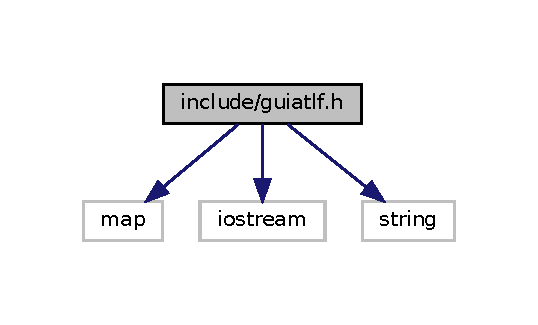
\includegraphics[width=258pt]{guiatlf_8h__incl}
\end{center}
\end{figure}
\subsection*{Clases}
\begin{DoxyCompactItemize}
\item 
class \hyperlink{classGuia__Tlf}{Guia\+\_\+\+Tlf}
\begin{DoxyCompactList}\small\item\em T.\+D.\+A. \hyperlink{classGuia__Tlf}{Guia\+\_\+\+Tlf} Una instancia {\itshape c} del tipo de datos abstracto {\ttfamily \hyperlink{classGuia__Tlf}{Guia\+\_\+\+Tlf}} es un objeto formado por una colección de pares \{(e11,e21),(e12,e22),(e13,e23),...,(e1n-\/1,e2n-\/1)\} ordenados por la el primer elemento del par denominado clave o key. No existen elementos repetidos. \end{DoxyCompactList}\item 
class \hyperlink{classGuia__Tlf_1_1iterator}{Guia\+\_\+\+Tlf\+::iterator}
\begin{DoxyCompactList}\small\item\em clase para iterar sobre la guia \end{DoxyCompactList}\end{DoxyCompactItemize}


\subsection{Descripción detallada}
\+: T\+DA guia de telefonos 


%--- End generated contents ---

% Index
\backmatter
\newpage
\phantomsection
\clearemptydoublepage
\addcontentsline{toc}{chapter}{Índice}
\printindex

\end{document}
